\documentclass[11pt,a4paper]{article}

\usepackage{fullpage}
\usepackage[margin=1in]{geometry}
\usepackage[utf8]{inputenc}

\usepackage{graphicx}
\graphicspath{ {images/} }

\usepackage[colorlinks = true,
            linkcolor = blue,
            urlcolor  = blue,
            citecolor = blue,
            anchorcolor = blue]{hyperref}

\begin{document}

\title{COSC3500 \\ 2D Orbital Simulation Report}
\author{Maxwell Bo (43926871)}
\date{August 17, 2018}
\maketitle

% Description of problem - readable and covers all salient points - /2
\subsection*{Description}

% Description of implementation - is coherent and has sufficient depth and detail - /5
\subsection*{Implementation}

% Why do you believe it is correct - /3
\subsection*{Correctness}

% Scaling or other performance discussion - /2
\subsection*{Performance \& Scaling}

The addition of the 
\texttt{-march=native} compiler flag, which enables the use of all CPU specific instructions, provided no recognizable improvement in running time.

The use of the GCC and Clang Profile-Guided Optimisation features provided no recognizable improvement in running time.

Distressingly, \texttt{-O0}, \texttt{-O1}, \texttt{-O2}, \texttt{-O3} showed no recognizable improvement in running time. \texttt{-Ofast} led to an -4\%-ish performance regression.


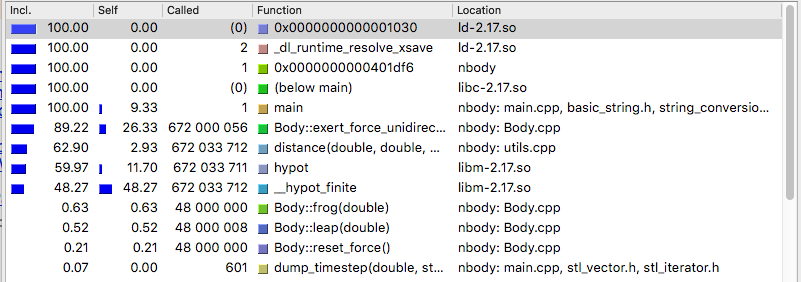
\includegraphics[width=\textwidth]{profile}

% The \texttt{exert_force_unidirectionally} method was an incredibly costly method, with an exclusive cost of 26.33\% of total running time.

Two performance fixes were divised.

\begin{lstlisting}
void Body::exert_force_unidirectionally(const Body& there) {
    double m1 = m;
    double m2 = there.m;
    double r = distance(x, y, there.x, there.y);
    double r2 = r * r;

    double F = (G * m1 * m2) / r2;

    double delta_x = there.x - x;
    double delta_y = there.y - y;

    // turn the displacement vector between our two points into a force vector
    // of the desired magnitude
    double scale_factor = F / r;

    Fx += delta_x * scale_factor;
    Fy += delta_y * scale_factor;
}
\end{lstlisting}

Here, we are recalculating 


gcc -g -lstdc++ -Wall -pedantic -Wextra -std=c++11 -lm -O3 -march=native Body.o
QuadTree.o main.o utils.o -o nbody
Barnes-Hut enabled: false
Leapfrog enabled: true
Total CPU time was 13.938825
12000001 simulation steps computed


\end{document}
